\documentclass[border=6pt]{standalone}
\usepackage{tikz}
\usepackage{pgfplots}
\pgfplotsset{compat=1.18}
\usetikzlibrary{arrows.meta,positioning,shapes.geometric,fit,backgrounds,calc,decorations.pathreplacing,patterns,pgfplots.groupplots}
\tikzset{
  blk/.style={rectangle, rounded corners=2pt, draw=black!70, thick, fill=blue!6,
              minimum height=8mm, minimum width=20mm, align=center, font=\small},
  io/.style={rectangle, rounded corners=6pt, draw=black!70, thick, fill=green!8,
             minimum height=8mm, align=center, font=\small},
  proc/.style={rectangle, draw=black!70, thick, fill=orange!10, minimum height=8mm,
               align=center, font=\small},
  dec/.style={diamond, aspect=2, draw=black!70, thick, fill=yellow!15, align=center, font=\footnotesize},
  warnbox/.style={rectangle, rounded corners=2pt, draw=red!60!black, thick, fill=red!7,
                  minimum height=8mm, align=center, font=\small},
  oklbox/.style={rectangle, rounded corners=2pt, draw=green!45!black, thick, fill=green!8,
                 minimum height=8mm, align=center, font=\small},
  ar/.style={-{Latex[length=2mm]}, thick},
  arl/.style={-{Latex[length=2mm]}, thick, dashed, draw=black!55},
  lbl/.style={font=\footnotesize\itshape, text=black!60},
}
\definecolor{good}{RGB}{34,139,34}
\definecolor{bad}{RGB}{178,34,34}
\definecolor{warn}{RGB}{218,165,32}
\definecolor{pesblue}{RGB}{0,45,98}
\definecolor{complete}{RGB}{30,125,79}
\definecolor{partial}{RGB}{176,106,0}
\definecolor{blocked}{RGB}{166,43,43}
% ---------------------------------------------------------------------------
% fig_coverage_vs_score -- coverage (fraction of the declared suite executed
% and natively graded) vs. availability of a quotable native score, all 14 lanes.
%
% Data sources (real, read from repo):
%   outputs/E1_E14_FINAL_RESULTS_2026-09-19.md
%       -> the final lane ledger; every x value and every annotation string
%   outputs/verification/LEDGER_CODE_CHECK_2026-09-19.json
%       -> machine check 11/11 PASS: E1 2/731, E8 1967/1967, E11 129/312
%          (129/311 sensitivity), E14 4426/4428 acc 0.5131043831902395,
%          E9 40 unique competitions of 75
%   primary receipts:
%       outputs/e4_banker_toolbench/official_repo_ff6db552/jobs/
%         btb-banking-tasks-tinker-bridge/result.json  -> 100/100 trials,
%         metrics mean 0.0 (all 100 in the 0.0 reward bucket)
%       outputs/e5_apex_agents/e5_exact_sequential_prefix_aggregate_2026-08-22.json
%         -> 7 natively scored of 480 (PARTIAL_EXACT, fixed prefix 0-10)
%       outputs/e7_binaryaudit/2026-08-22_e7_paid_attempt_receipt.json +
%         split_manifest.json -> 1 attempted of 46 constructed rows
%       outputs/public_portfolio_2026-09-05/canonical_before_report_v15/results.json
%         -> E8 1967, E10 97, E11 312, E6 0/812
%   E13 provenance note: "13/255 episodes" is ledger text; its named source
%   (outputs/PES_Phase2_Review_2026-09-12/finish/e13_continuation/decision_v11/
%   DECISION.md) records 13 completed episodes among 29 started exclusions with
%   full-255 scoring disabled, while the 2026-09-05 v15 portfolio records
%   0/255 model episodes.  Either way the lane carries no native score, which
%   is where the point is plotted.
% ---------------------------------------------------------------------------
\begin{document}
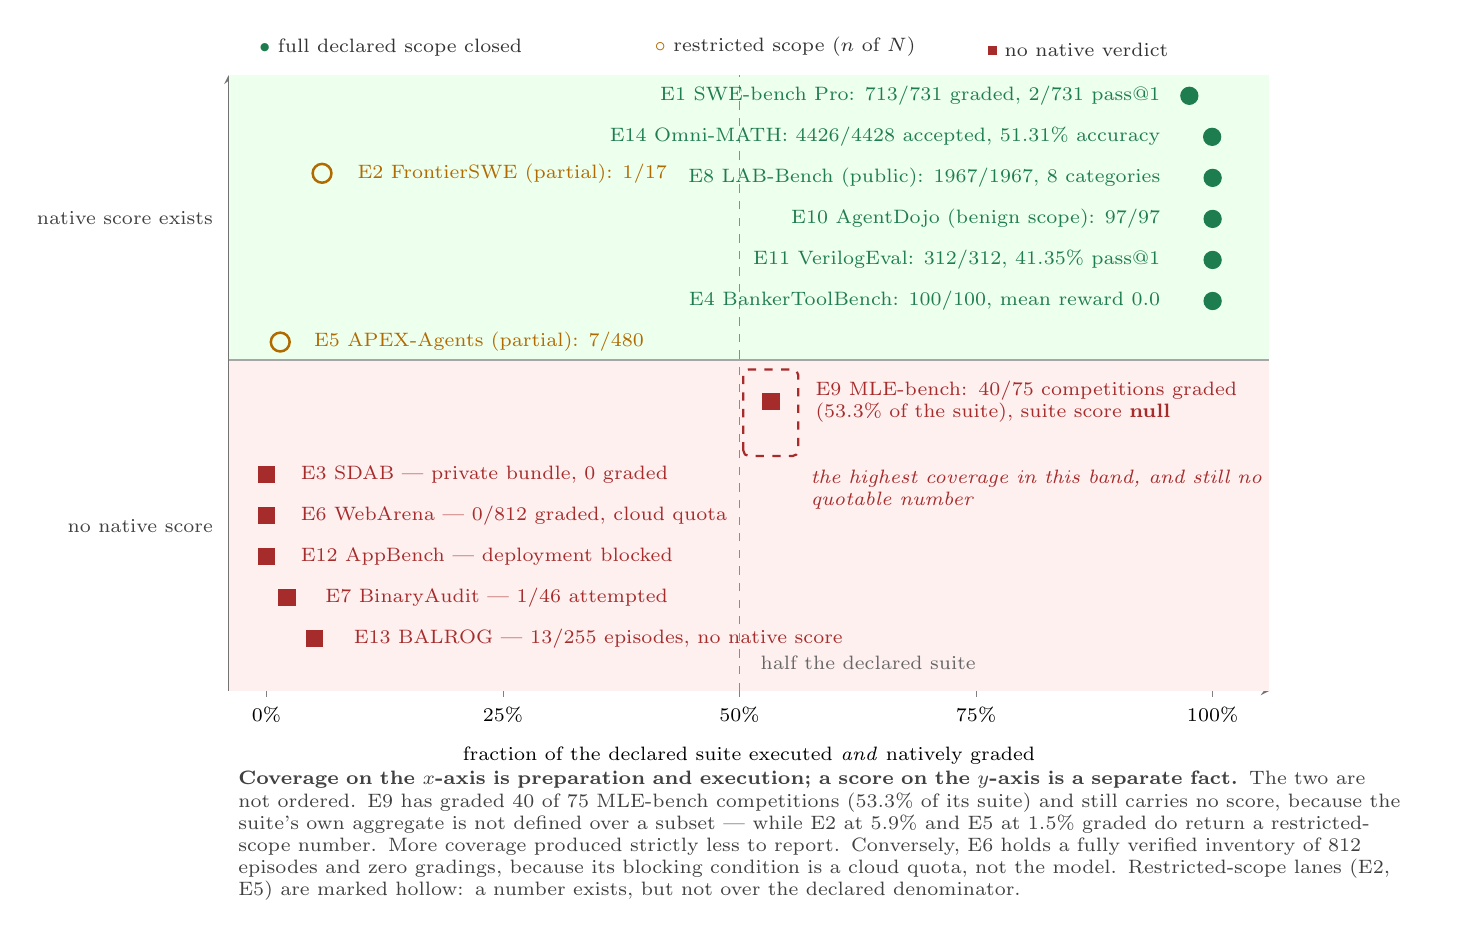
\begin{tikzpicture}
\begin{axis}[
  width=14.8cm, height=9.4cm,
  xmin=-4, xmax=106, ymin=-0.85, ymax=1.85,
  xtick={0,25,50,75,100},
  xticklabel={\pgfmathprintnumber{\tick}\%},
  ytick={-0.125,1.225},
  yticklabels={no native score, native score exists},
  ytick style={draw=none},
  every y tick label/.style={font=\scriptsize, align=right, text=black!75},
  xlabel={\scriptsize fraction of the declared suite executed \emph{and} natively graded},
  every axis x label/.style={at={(0.5,-0.075)},anchor=north},
  axis lines=left, axis line style={black!55},
  tick label style={font=\scriptsize},
  clip=false,
]

% ---------- regime bands: y encodes only whether a verdict exists ----------
\fill[red!6]  (axis cs:-4,-0.85) rectangle (axis cs:106,0.60);
\fill[green!7] (axis cs:-4,0.60)  rectangle (axis cs:106,1.85);
\draw[black!35, thick] (axis cs:-4,0.60) -- (axis cs:106,0.60);

% half-the-suite reference
\draw[dashed, black!45] (axis cs:50,-0.85) -- (axis cs:50,1.85);
\node[lbl, anchor=south west, font=\scriptsize] at (axis cs:51.2,-0.80)
  {half the declared suite};

% ================= BAND: a native verdict exists =================
% ---- full declared scope closed ----
\addplot[only marks, mark=*, mark size=3.1pt, color=complete]
  coordinates {(97.54,1.76) (99.95,1.58) (100,1.40) (100,1.22) (100,1.04) (100,0.86)};
\node[font=\scriptsize, anchor=east, color=complete] at (axis cs:95.5,1.76)
  {E1 SWE-bench Pro: $713/731$ graded, $2/731$ pass@1};
\node[font=\scriptsize, anchor=east, color=complete] at (axis cs:95.5,1.58)
  {E14 Omni-MATH: $4426/4428$ accepted, $51.31\%$ accuracy};
\node[font=\scriptsize, anchor=east, color=complete] at (axis cs:95.5,1.40)
  {E8 LAB-Bench (public): $1967/1967$, 8 categories};
\node[font=\scriptsize, anchor=east, color=complete] at (axis cs:95.5,1.22)
  {E10 AgentDojo (benign scope): $97/97$};
\node[font=\scriptsize, anchor=east, color=complete] at (axis cs:95.5,1.04)
  {E11 VerilogEval: $312/312$, $41.35\%$ pass@1};
\node[font=\scriptsize, anchor=east, color=complete] at (axis cs:95.5,0.86)
  {E4 BankerToolBench: $100/100$, mean reward $0.0$};

% ---- restricted scope only: a score, but over part of the suite ----
\addplot[only marks, mark=o, mark size=3.4pt, line width=0.9pt, color=partial]
  coordinates {(5.88,1.42) (1.46,0.68)};
\node[font=\scriptsize, anchor=west, color=partial] at (axis cs:8.6,1.42)
  {E2 FrontierSWE (partial): $1/17$};
\node[font=\scriptsize, anchor=west, color=partial] at (axis cs:4.0,0.68)
  {E5 APEX-Agents (partial): $7/480$};

% ================= BAND: no native verdict =================
\addplot[only marks, mark=square*, mark size=2.9pt, color=blocked]
  coordinates {(0,0.10) (0,-0.08) (0,-0.26) (2.17,-0.44) (5.10,-0.62) (53.33,0.42)};
\node[font=\scriptsize, anchor=west, color=blocked] at (axis cs:2.6,0.10)
  {E3 SDAB --- private bundle, $0$ graded};
\node[font=\scriptsize, anchor=west, color=blocked] at (axis cs:2.6,-0.08)
  {E6 WebArena --- $0/812$ graded, cloud quota};
\node[font=\scriptsize, anchor=west, color=blocked] at (axis cs:2.6,-0.26)
  {E12 AppBench --- deployment blocked};
\node[font=\scriptsize, anchor=west, color=blocked] at (axis cs:5.2,-0.44)
  {E7 BinaryAudit --- $1/46$ attempted};
\node[font=\scriptsize, anchor=west, color=blocked] at (axis cs:8.2,-0.62)
  {E13 BALROG --- $13/255$ episodes, no native score};
\node[font=\scriptsize, anchor=west, align=left, color=blocked, text width=5.6cm]
  at (axis cs:57.0,0.42)
  {E9 MLE-bench: $40/75$ competitions graded\\ ($53.3\%$ of the suite), suite score \textbf{null}};
\draw[blocked, thick, rounded corners=2pt, dashed]
  (axis cs:50.4,0.18) rectangle (axis cs:56.2,0.56);

% mark the E9 gap explicitly
\node[font=\scriptsize\itshape, anchor=north west, color=blocked, text width=6.2cm]
  at (axis cs:56.5,0.16)
  {the highest coverage in this band, and still no quotable number};

% ================= legend =================
\node[font=\scriptsize, anchor=south west, text=black!80] at (axis description cs:0.02,1.015)
  {\textcolor{complete}{$\bullet$}\ full declared scope closed};
\node[font=\scriptsize, anchor=south west, text=black!80] at (axis description cs:0.40,1.015)
  {\textcolor{partial}{$\circ$}\ restricted scope ($n$ of $N$)};
\node[font=\scriptsize, anchor=south west, text=black!80] at (axis description cs:0.72,1.015)
  {\textcolor{blocked}{\rule[0.15ex]{3.4pt}{3.4pt}}\ no native verdict};

% ================= reading note =================
\node[anchor=north west, align=left, font=\scriptsize, text=black!75, text width=15.0cm]
  at (axis description cs:0.0,-0.115)
  {\textbf{Coverage on the $x$-axis is preparation and execution; a score on the $y$-axis is a
   separate fact.} The two are not ordered. E9 has graded $40$ of $75$ MLE-bench competitions
   ($53.3\%$ of its suite) and still carries no score, because the suite's own aggregate is not
   defined over a subset --- while E2 at $5.9\%$ and E5 at $1.5\%$ graded do return a
   restricted-scope number. More coverage produced strictly less to report. Conversely, E6 holds a
   fully verified inventory of $812$ episodes and zero gradings, because its blocking condition is
   a cloud quota, not the model. Restricted-scope lanes (E2, E5) are marked hollow: a number
   exists, but not over the declared denominator.};

\end{axis}
\end{tikzpicture}
\end{document}
